%\cleardoublepage

\begin{figure}
\begin{center}
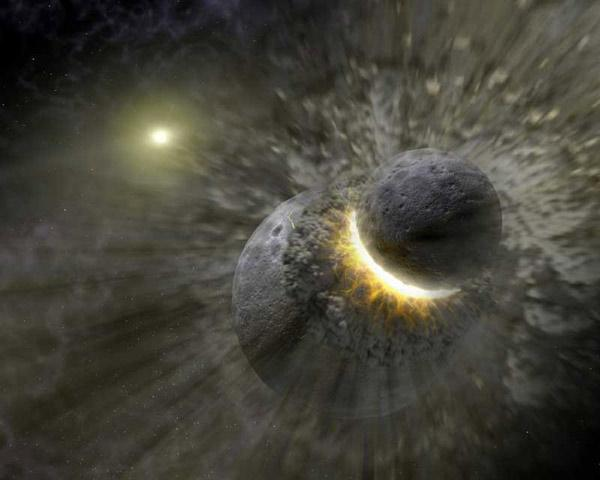
\includegraphics[scale=0.6]{01figs/01planet-collision.jpg}
\caption{Artists impression of the Moon forming giant impact. Image courtesy of NASA/JPL-Caltech}
\label{ch01_fig01}
\end{center}
\end{figure}


\chapter{Introduction}
\label{ch01}
\graphicspath{{./01figs/}}

The field of planet formation lead a neglected existence besides related fields like stellar formation or cosmology for a long time. While telescopes allowed mankind to observe stars beyond the solar system for several centuries, the knowledge about planets has long been limited to the ones in our own system. The relative small luminosity of planets compared to stars makes it even today almost impossible to directly detect planets even for stars in our neighborhood. Without any further known systems, the question wether planet formation is a common process alongside of stellar formation remained non answerable question. But the common wisdom was, that the solar system is a typical result of planet formation and that hypothetical extrasolar systems should look similarly. This is no surprise, as planet formation models primarily aimed at explaining the solar system.

The discovery of the first extrasolar planet \emph{51 Pegasi b} around a solar-type star by \cite{1995Natur.378..355M} caused an overnight revolution in the field. 
Before this discovery, nobody deemed it possible that a Jupiter-mass planet could exist as close as $0.05 AU$ to its host star. As of July 2011, ongoing ground- and space-based observations have discovered more than 560 extrasolar planets. All of them are relatively massive and close-in, more resembling the originally observed \emph{51 Pegasi b} than the planets in our own solar system. This is primarily an effect of observational bias, favoring the detection of massive, close-in planets. Nevertheless, a model of planet formation also has to explain those systems.

Collisions between bodies of various sizes are an important process during all stages of planet formation. A collision consists of two macroscopic bodies, the larger body termed the \emph{target} and the smaller body called the \emph{impactor} approaching each other and resulting in a collisional outcome depending what the various parameters of the collision are. When the target is considerably larger than the impactor, a collision is also often called an impact. Collisions occur at various stages during planet formation, with mass and size ranges varying several tens of magnitudes from dust grains up to Jupiter sized planets. This thesis covers different types of collisions all modeled with the same type of method described in detail in chapter \ref{ch02}. The following brief overview on planet formation helps in putting these different types of collisions in context within planet formation.

According to the current understanding of planet formation, the formation process of a planetary system can be divided into different stages: A part of a giant molecular cloud, composed of gas (mainly H \& He) and dust, collapses and starts to form a rotating disk due to the conservation of angular momentum. When density and pressure are large enough in the center, hydrogen burning starts and a new star is born. Over time, what resembles a rotating lump of gas first, changes disk with decreasing pressure, density and temperature as a function of the distance to the star.

Due to the radial pressure gradient, the gas rotates with a sub-keplerian velocity around the star. In the vertical direction relative to the disks midplane, there is also a positive pressure gradient towards the midplane. While the dust is tightly coupled to the rotation of the gas around the star, it is pressureless in itself and therefore settles towards the disks midplane over a timescale of $10^4$ years. The $\mu m$-sized dust starts to coagulate due to strong van-der-Waals forces into larger grains \citep{2010A&A...513A..56G}. As the grains grow towards bigger, planetesimals their relative strength becomes smaller as inter-molecular forces increase $\sim r^2$ while intertial forces increase with $\sim r^3$. With the diameter approach the \emph{meter-sized barrier}, further growth of the solid is stopped and erosion begins \cite{Benz1999Icar..142....5B}.

How this barrier can be overcome is still a unknown. Recent suggestions have been the trapping of dust in vortices, either caused by magneto-rotational-instability \citep{Johansen:2007p37} or by turbulence in general \citep{2008ApJ...686.1292I}. In those scenarios, the trapped dust instantly collapses under its self-gravity into \emph{Ceres} sized objects ($\approx 10^{-4} \ME$). In this regime, gravity becomes strong enough to hold together those objects and further mass is accreted. Due to gravitational focussing, the zone where those bodies accreted mass from increases with their mass and leads to \emph{runaway accretion}. During this stage, the amout of gas in the disk already has decreased, either by accretion onto the central star or due to photo-evaporation due to the young stars UV radiation.

The growing planetesimals now turn into planetary embryos and become a victim of their own success: When an embryo reaches a mass $\approx 100\times$ larger than the typical planetesimal mass in its vicinity, this feeding zone is being emptied and the accretion rate goes down again. Neighboring embryos can catch up and the \emph{oligarchic} accretion regime kicks in \citep{1993Icar..106..210I, 2010ApJ...714L.103O}.

The individual embryos reach similar masses and are orderly spaced according to their feeding-zones. The remaining small planetesimals stabilize the orbits of the embryos through dynamical friction, while their own eccentricities and inclinations are pumped up, leading to slow removal of the planetesimals due to accretion onto embryos, loss into the central star or due to ejection. WIth the removal of the planetesimals and almost no gas around, the embryos becomes unstable again and eventually get on crossing orbits. The resulting two-body interactions chaotically re-arrange the embryos in the disk and lead to collisions in some cases \cite{Chambers:2001p2105, Chambers:2004p4098}. With all embryos occupying the same mass regime, these collisions are called similar-sized and lead to various outcomes \cite{Asphaug:2010p3539}. Such collisions and their outcomes are discussed in detail in chapter \ref{ch03}. Work on modeling the stage between the formation embryos and their final accretion into proto-planets \cite{Chambers:2001p2105, 2006Icar..184...39O} often makes simplified assumptions about these similar-sized collisions. The data provided in chapter \ref{ch03} permits such models to incorporate a more realistic collision handling and model this stage of planet formation more precisely.

Similar-sized collisions alter bodies in a profound way: Properties like composition, bulk density \citep{Benz:1988p3336} or the rotation can be changed by this collisions. They are also believed to trigger core formation \cite{1992Icar..100..326T}. 

Consequently, the final properties of terrestrial planets are heavily influenced by the last massive collision they underwent: Primordial atmospheres can be removed \cite{2002DPS....34.2804A} or the planet can be depleted of its volatiles \citep{2001E&PSL.192..545H}.

Another interesting effect of such collisions is satellite formation. Along with the Pluto-Charon binary system \cite{Canup:2005p1987}, the Earths Moon is most probably a direct outcome of a late giant collision between the proto-Earth and a roughly Mars sized body \citep{1975Icar...24..504H, 1976LPI.....7..120C, 1987Icar...71...30B, Canup:2001p1861}. In chapter \ref{ch05}, we look into a model explaining the Moons formation with an alternative impact scenario.

The growth of solid embryos is not only important for the formation of terrestrial planet, but also delivers the cores required for giant planet formation \citep{1996Icar..124...62P}. Understanding the timescales of embryo growth is crucial, as they have to becomes massive enough to start to accrete gas, before the gas disk vanishes. 

With the late heavy bombardment marking the last major event in the solar systems history \citep{2005Natur.435..466G}, planet formation as a process has finished. Nevertheless, impacts of small remnants for example from the asteroid or the Kuiper belt onto planets and their moons still take place. While not delivering substantial mass relative to the target body, the craters such impacts leave give clues about the rheology and age of planetary surfaces. Chapter \ref{ch04} presents modeling work on martian craters which have been observed only months after their formation \cite{2009Sci...325.1674B}. 





%statistical results for evolution codes, to understand planet formation in general 

especially terrestrial planet formation 
%\cite{Lisse:2009p3131} -> chapter 3

cratering collisions: helpful for dating 
application of impacts mars -> chapter 4


method side: SPH as a robust method for collisions, thermodynamics are important

%SPH has been used for single, large cases mainly \cite{2005Natur.435..629S}

progress in computational methods and computing power allows massively parallel 




%\section{Motivation}
%collisions as event between two bodies
%cratering to similar sized collisions
%importance in solar system formation
%outcomes give clues 
%solar system dimensions
% refer to chapters: 

% motivation for simulating collisions
% introduce collision basics and terms
% give examples of collisions

% check Augustins Diss

%\section{Collision basics}
%introduce terms: impactor, target, impact velocity, impact angle

\bibliographystyle{plainnat}
\bibliography{bibliography}
